\chapter{Results}
\section{Achievements}
The main goal of this project described below has been met. This goal contained a lot of sub-goals which ultimately dwell down to one thing: converting OSM data into the NeTEx format.\\
\newline
Integrating OpenStreetMap with Public Transport Network Format "NeTEx" using the JOSM editor:
\begin{itemize}
	\item{Create a JOSM plugin in Java for converting OSM data into NeTEx.}
	\begin{itemize}
		\item{Create a JOSM friendly plugin.}
		\item{Convert and export the loaded OSM data of JOSM into a single .XML file using the generated NeTEx Java model.}
		\item{Fix data inconsistency problems by identifying and saving missing tags/information}
		\item{Log the warning messages created while converting the data in the JOSM map layer relative elements}
		\item{Have the plugin deployed in a single \textit{.jar} file.}
	\end{itemize}
	\item{Translate the NeTEx XML schema into a Java model.}
	\item{Publish the plugin in the official JOSM plugins repository.}
\end{itemize}
\newpage
\section{Product Results}
The only type of data needed to deliver the results for the plugin is only OSM data. This data is converted and checked carefully during the conversion in order to find out what it really represents in transport and in the NeTEx format. The simplicity of running this plugin and converting the loaded OSM data into NeTEx is a powerful attribute that it possesses.\\
\newline
Here's a bus stop, consisting of two platforms (on both sides) and the way it looks on JOSM (with the OSM data):
\begin{figure}[H]
	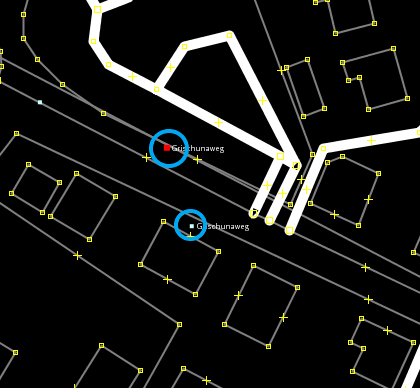
\includegraphics[width=\linewidth]{./Images/Results/results_osm_example_1.png}
	\caption{An example of a bus stop in OpenStreetMap (Location - Chur, Switzerland)}
\end{figure}
And its tags:
\begin{figure}[H]
	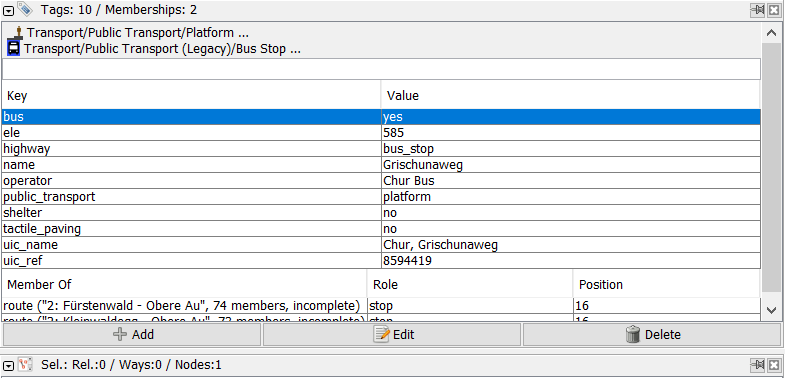
\includegraphics[width=\linewidth]{./Images/Results/results_osm_example_2.png}
	\caption{An example of a bus stop tags in OpenStreetMap (Location - Chur, Switzerland)}
\end{figure}
And here's that same bus stop, after being converted to NeTEx using this plugin:
\begin{minted}[tabsize=2,breaklines]{xml}
<StopPlace id="ch:1:StopPlace:8594419">
<Name>Grischunaweg</Name>
<PrivateCode>org:osm:node:6104311285</PrivateCode>
<Centroid>
<Location>
  <Longitude>9.5139936</Longitude>
  <Latitude>46.8527028</Latitude>
</Location>
</Centroid>
<AccessibilityAssessment>
<limitations>
  <AccessibilityLimitation>
    <WheelchairAccess>false</WheelchairAccess>
  </AccessibilityLimitation>
</limitations>
</AccessibilityAssessment>
<PublicCode>8594419</PublicCode>
<StopPlaceType>onstreetBus</StopPlaceType>
<quays>
<Quay id="ch:1:Quay:8594419:6104311285">
  <PrivateCode>org:osm:node:6104311285</PrivateCode>
  <Centroid>
    <Location>
      <Longitude>9.5139936</Longitude>
      <Latitude>46.8527028</Latitude>
    </Location>
  </Centroid>
  <PublicCode>6104311285</PublicCode>
  <QuayType>busStop</QuayType>
</Quay>
<Quay id="ch:1:Quay:8594419:2446137123">
  <PrivateCode>org:osm:node:2446137123</PrivateCode>
  <Centroid>
    <Location>
      <Longitude>9.5139237</Longitude>
      <Latitude>46.8528536</Latitude>
    </Location>
  </Centroid>
  <PublicCode>2446137123</PublicCode>
  <QuayType>busStop</QuayType>
</Quay>
</quays>
</StopPlace>
\end{minted}
\begin{itemize}
\item{The \textit{StopPlace} node represents the bus stop and contains all of the other data such as: ID, name, location, public code, its type etc.}
\item{The \textit{Quay} node represents the platform of the bus stop along with the other attributes such as: ID, location, platform type etc.}
\item{The \textit{AccessibilityAssessment} node represents accessibility features for the bus stop, in this case only whether it is accessible with a wheelchair or not, and if no info about that is found from the tags, it falls back to a "false" value.}
\end{itemize}
More information on what all of the NeTEx objects represent can be found on the official NeTEx schema documentation.
\newpage
\section{Reflection}
I have never used OpenStreetMap before, let alone JOSM. This project made me learn a lot of key factors that drive OSM and make OSM such a successful project for the community. It also improved my ability to work in an open-source project and know the approaches that are used by developers when developing open-source projects.\\
\newline
I wasn't very informed about transport data either and never heard of NeTEx before either, so a combination of OSM and NeTEx was very beneficial for me. It is also the first time I have created something that is similar to converting data of a format into a completely different format. The process was a tough challenge but also a very rewarding one.\\
\newline
I have had a lot of experience with working with Java before, but not that much experience of coding in open-source projects where you have to code by following "protocol". I had to do a lot of research within the code, but after a while, I understood how the whole thing worked and then after that, everything in the code made sense and was straight-forward to reach in the code.\\
\newline
I had also never worked with an XML binding framework before either and it was wonderful to see how such things are made possible in the programming world; without such frameworks, this would be hardly possible! A lot of technologies and approaches used here were a new experience for me and even though it was overwhelming sometimes, it was definitely worth it!